\chapter{Východiská}
\label{kap:vyc} % id kapitoly pre prikaz ref

\section{Úvod do problematiky}

Problém hľadania optimálnej cesty je veľmi rozšíreným problémom nie len v doprave. Doteraz bolo navrhnutých množstvo algoritmov, metód a techník na vyriešenie tohto problému. Pri hľadaní optimálnej trasy vo verejnej doprave je dobré si najskôr ujasniť, čo  výraz optimálna cesta znamená.

Najlepšie zhrnutie podproblémov, ktoré môžu nastať sme postrehli v článku \cite{circular}. 
Autori analyzujú ich návrh v najzložitejšom systéme verejnej dopravy - v Hongkongu. Pre verejnú dopravu je praktickejšie navrhnúť viac alternatívnych ciest. Najbežnejšie používateľské preferencie sú:
\begin{itemize}
\item{minimálny čas}
\item{minimálne poplatky}
\item{minimálny počet prestupov}
\item{minimálna vzdialenosť peších prestupov}
\end{itemize}
Ďalej si treba uvedomiť, že môžu existovať rôzne typy liniek - jednosmerné alebo okružné a taktiež linky závislé na čase - denné, nočné alebo víkendové linky. Vzhľadom na rôzne požiadavky existuje viacero potenciálnych riešení. Neexistuje totiž všeobecne dokonalý spôsob na hľadanie optimálnej cesty, ktorý sedí pre každú verejnú dopravu, najmä kvôli rozloženiu zastávok.

Bratislavská verejná doprava má rôzne typy dopravných prostriedkov (autobus, trolejbus a električka), čo tiež predstavuje určitý problém. Pri prestupoch treba zohľadniť aj pešie presuny. Dopravná sieť, ktorú budeme modelovať v našej práci je teda multimodálna. Multimodálna sieť je definovaná ako kombinácia dvoch a viacerých dopravných prostriedkov na prepravu cestujúcich alebo tovaru z počiatočného miesta na miesto určenia \cite{timedependent}.

Ďalším kľúčovým problémom sú podľa zadania reálne dáta. Bude potrebné vyriešiť, ako sa vysporiadať so spracovaním reálnych dát. Kľúčový bude výber dátovej štruktúry na ich spracovanie, ako aj nájdenie vhodného časovo závislého algoritmu.

Sumarizáciou nášho problému je, ako sa vysporiadať s dynamickými dátami, alternatívnymi cestami, viacerými módmi, navigáciou z iného miesta ako zo zástavky. Ďalej chceme vyhovieť používateľským preferenciám, ako je minimálny čas, minimálny počet prestupov a minimálna vzdialenosť peších prestupov. Neposledným problémom je návrh architektúry systému.

V tejto kapitole ďalej opíšeme často skloňované algoritmy pri téme multimodálneho časovo závislého vyhľadávania vo verejnej doprave a priblížime výskumy, ktoré riešili podobné problémy ako my.

\section{Dijkstrov algoritmus}
Najznámejším algoritmom hľadania najkratšej cesty v orientovanom, kladne ohodnotenom grafe je Dijkstrov algoritmus. Algoritmus vie nájsť najrýchlejšiu cestu medzi dvomi danými vrcholmi. Známejšou verziou Dijkstrovho algoritmu je hľadanie najkratšej cesty z jedného vrcholu do všetkých ostatných vrcholov v grafe. 

Rozhodujúcou hodnotou je vzdialenosť vrcholu $d(n)$, ktorá predstavuje dĺžku cesty od štartovného vrcholu po vrchol $n$, pričom cesta vedie cez aktuálny vrchol.
Pre štartovný vrchol sa vzdialenosť $d(n) = 0$ a všetky ostatné vrcholy majú hodnotu $d(n) = \infty$. Na začiatku je štartovný vrchol označený ako aktuálny. Pri každej iterácii algoritmus preskúma všetky susedné vrcholy aktuálneho vrcholu. Pre každý susedný vrchol prepočíta hodnotu $d(n)$. Ak je táto hodnota menšia ako predtým zaznamenaná, prepíše ju menšou hodnotou. Ďalej algoritmus označí aktuálny vrchol ako navštívený. Tým pádom sa tento vrchol už nebude viac prehľadávať. Aktuálnym vrcholom sa stane zatiaľ nenavštívený vrchol s najmenšou hodnotou $d(n)$. 

Ak hľadáme cestu medzi dvomi konkrétnymi vrcholmi, algoritmus končí, keď bol konečný vrchol označený ako navštívený. Inak končí, ak neexistujú žiadne nenavštívené vrcholy alebo majú všetky hodnotu $d(n) = \infty$.

Časová zložitosť Dijkstrovho algoritmu je kvadratická
$\mathcal{O}(|V|)$, kde $V$ je množina všetkých vrcholov v grafe. V pôvodnej verzii, kde hľadáme najkratšiu cestu len medzi dvomi vrcholmi, môže algoritmus bežať rýchlejšie.

Nevýhodou algoritmu je veľký prehľadávaný priestor. Existuje viacero algoritmov, ktoré vznikli modifikáciou Dijkstrovho algoritmu. Napríklad Bellman-Fordov algoritmus, ktorý sa vie vysporiadať aj so zápornými hranami alebo A*, ktorý využíva heuristiku na zmenšenie prehľadávaného priestoru. 

\section{A* algoritmus}
A* algoritmus je grafový optimálny algoritmus na nájdenie najkratšej cesty medzi dvoma bodmi. Vznikol kombináciou heuristických a formálnych prístupov. Udržuje strom ciest, ktoré majú začiatok v začiatočnom vrchole a predlžuje tieto cesty po jednej hrane. Pri každej iterácii sa rozhodne, ktorú z ciest rozšíri. Algoritmus sa skončí, ak už neexistuje žiadna cesta na rozšírenie alebo pri dosiahnutí koncového vrcholu. Pri prehľadávaní používa stratégiu najskôr najlepšieho. Heuristika, ktorá sa využíva na vyhodnotenie vzdialeností, je funkcia
\begin{equation}
f(n) = g(n) + h(n), 
\end{equation}
kde $g(n)$ predstavuje hodnotu cesty zo začiatočného vrcholu do vrcholu $n$ a $h(n)$ je heuristická funkcia, ktorá odhaduje najkratšiu cestu z vrcholu $n$ do koncového vrcholu.

Najčastejšie používaná heuristická funkcia na odhadovanie vzdialenosti je Euklidovská vzdialenosť.
Heuristika je prípustná, ak nikdy neprecení skutočné náklady na dosiahnutie cieľa. Potom je zaručené, že algoritmus A* vráti najkratšiu cestu, ak taká v grafe existuje.

Časová zložitosť A* algoritmu závisí od zvolenej heuristiky. V najhoršom prípade je zložitosť algoritmu exponenciálna, v najlepšom prípade môže byť polynomiálna.

\section{Časovo závislý multimodálny algoritmus}

Článok \cite{timedependent} navrhuje časovo závislý algoritmus hľadania najkratšej cesty pre multimodálnu dopravnú sieť, pričom využíva A* algoritmus. Navrhnutý algoritmus hľadá len jednu cestu medzi štartovným a koncovým vrcholom. Pre zrýchlenie behu A* algoritmu navrhujú jeho optimalizáciu založenú na vypočítaní virtuálnej cesty, ktorá predstavuje Euklidovskú vzdialenosť zo štartovného do koncového vrcholu. 

Majme graf $G = (V, E, M)$, kde $V$ je množina vrcholov, $E$ je množina hrán a $M$ je množina módov. Hrana $e_i = (v_i, v_j, m_i)$ je cesta z vrcholu $v_i$ do $v_j$ použitím módu $m_i$. Vrchol, kde sa menia módy je prestupný vrchol. Ďalej definujú čas prestupu ako súčet:
\begin{itemize}
\item{času potrebného na prestup medzi dvomi zastávkami}
\item{času potrebného na čakanie na prestupný mód}
\item{času, ktorý stojí mód na zastávke (týka sa skôr prímestskej dopravy)}
\end{itemize}

Preto je potrebné pridať ďalšie prestupné hrany s tým, že ohodnotenie nebude statické, ale bude to funkcia $cost_{transfer}()$ závislá od času. Na vytvorenie modelu sú navrhnuté 2 prístupy: time-expanded model a time-dependent model.

\subsection{Time-expanded model}
Time-expanded model rozdelí čas na konečný počet intervalov a pre každý interval zduplikuje vrchol. Každá udalosť na každej stanici je modelovaná ako vrchol. Model je vhodný pre siete založené na cestovných poriadkoch. Je teda vhodný pre verejnú dopravu. Ľahko sa modeluje, ale vyžaduje veľa pamäte a vykonávanie dotazov je pomalé.

\subsection{Time-dependent model}
\textit{Time-dependent} model má klasickú topológiu. Počet vrcholov vo výslednom modeli je rádovo menší ako v \textit{time-expanded} modeli. Okrem iného je tento model aj efektívnejší. 

Pre každú zastávku $p$ je do modelu vložený \textit{station node}. Navyše pre každú zastávku $p$ v linke $r$ je vytvorený ďalší vrchol \textit{route node} $r_p$. \textit{Route nodes} sú spojené so \textit{stations nodes} hranami s konštantným ohodnotením. Toto ohodnotenie predstavuje čas potrebný na prestup. Jazda vozidla \textit{t} je definovaná ako postupnosť zastávok, ktoré vozidlo navštevuje podľa daného cestovného poriadku. Jazdy, ktoré pozostávajú z rovnakých vrcholov sú zoskupené do liniek. \textit{Route nodes}, ktoré patria jednej linke sú spojené hranou , ktorej hodnotou je funkcia. Hoci je takto vytvorený model menší, pre algoritmy je komplikovanejší. Ťažko sa na ňom vykonávajú dotazy v prípade, že je potrebné brať do úvahy prestupy.


\subsection{Navrhovaný algoritmus}

Navrhovaný algoritmus hľadá cestu cez vrcholy, ktoré sú blízko virtuálnej cesty. Parameter $d$ predstavuje šírku prehľadávaného priestoru a môže byť navýšený o ďalší parameter $\Delta d$. Definujeme parametre:
\begin{itemize}
\item{virtuálna cesta ($st$) – Euklidovská vzdialenosť z $s$ do $t$} a zároveň dolné ohraničenie prehľadávaného priestoru
\item{vzdialenosť $d$ - priemerná vzdialenosť všetkých vrcholov k virtuálnej ceste a predstavuje horné ohraničenie prehľadávaného priestoru}
\item{$d_{max}$ – vzdialenosť najvzdialenejšieho vrcholu od virtuálnej cesty}
\item{$\Delta d$ – priemerná vzdialenosť od všetkých vrcholov ku všetkým susedom}
\end{itemize}

$G = (V, E, M, T)$ multimodálny časovo závislý graf, kde $T$ je množina $travels$.
Nech hrana $e = (v, v’)_m$ má časovo závislú hodnotu $c_e(t)$, $travel$ pre hranu $e$ je definovaný ako dvojica $travel_e = (t, t’)$, kde $t$ je čas odchodu z $v$ a $t’$ je čas príchodu do $v’$.

Algoritmus funguje nasledovne:
\begin{enumerate}
\item Vypočítame: $D = dist(s,t)$, $d$ a $\Delta d$. Prehľadávaný priestor ma rozmery $(2d,D)$.
\item Začneme vytvárať cestu tak, že hľadáme vrchol $v_i$, ktorý spĺňa podmienku \\$dist(v_i, st) \leq d$. Ak nevieme nájsť žiadneho takého kandidáta, navyšujeme $d$ o $\Delta d$, až kým nejakého nenájdeme.
\item V každej ďalšej iterácii po vybratí vrcholu $v_i$ aplikujeme funkciu multimodálneho časovo závislého algoritmu hľadania najkratšej cesty na nájdenie ďalšieho kandidáta.
\item Ak sme prehľadali všetky vrcholy v grafe a nezostavili sme najkratšiu cestu, začneme prehľadávať odznovu s väčším prehľadávaným priestorom.
\end{enumerate}


\section{Optimalizačné metódy}
V tejto sekcii spomenieme ďalšie optimalizačné metódy, ktoré obmedzujú prehľadávanie použitím grafových algoritmov hľadania najkratšej cesty.

\subsection{Minimalizácia prehľadávaného priestoru}

V článku \cite{alternate} sa autori snažia nájsť spôsob, ako efektívne vypočítať najkratšiu cestu a tak odľahčiť cesty od dopravných zápch. Navrhujú algoritmus na nájdenie najkratšej alternatívnej cesty s minimálnym potrebným výpočtovým časom. Alternatívna cesta sa hľadá nasledovne: 
Vypočítame kapacitu cesty $RC$ a obsadenosť cesty $RO$, ktoré potrebujeme na výpočet indexu zápchy $CI$. Ak index zápchy je väčší ako $0.6$, vyhodnotíme alternatívnu najkratšiu cestu. Bol navrhnutý vzorec na výpočet kapacity cesty $RC$, obsadenosti cesty $RO$ a indexu zápchy $CI$. 

$$RC = L \cdot N,$$ kde L je dĺžka úseku cesty a N je počet jazdných pruhov. 

$$RO = \sum_{i=1}{N} A_i,$$ kde $A_i$, predstavuje dĺžku $i-teho$ vozidla na danom úseku cesty.

$$CI = \frac{RO}{RC}$$

Pre nás zaujímavý je ich prístup k vyhodnoteniu najkratšej cesty a k minimalizácii grafu. Minimalizáciu grafu prebieha nepretržite. Vždy, keď zvažujeme ďalší susedný vrchol, definujeme nový \textit{bounding box} a tým odstránime nadbytočné vrcholy, ktoré pri výpočte nehrajú žiadnu rolu.

Na začiatku potrebujeme vymodelovať graf mesta, kde sú vrcholy popísané zemepisnou šírkou a výškou a hrany sú ohodnotené reálnou vzdialenosťou medzi jednotlivými vrcholmi. Graf je opísaný tabuľkovou maticou a reprezentovaný graficky. Keď poznáme štartovný a koncový vrchol, vytvoríme si tabuľku všetkých vrcholov, ich súradníc a vzdialeností do štartovného vrcholu a koncového vrcholu. Podľa súradníc vieme vypočítať vzdialenosti medzi jednotlivými vrcholmi. Následne vygenerujeme grafickú reprezentáciu tejto tabuľky. 

\subsubsection{Bounding box}
Majme dopravnú sieť tvorenú 26 vrcholmi a majme začiatočný a koncový vrchol. \textit{Bounding box} je na začiatku vytvorený medzi štartovným a koncovým vrcholom, ako je ukázané na obrázku \ref{fig:boundingBoxReal}. \textit{Bounding box} zredukuje sieť na 8 vrcholov, čím zredukuje prehľadávaný priestor, výpočtovú cenu a čas. Ďalšiu redukciu vieme dosiahnuť, ak nakloníme bounding box tým spôsobom, že spojnica začiatočného a koncového vrcholu bude osou boxu, ako môžeme vidieť na obrázku \ref{fig:boundingBoxRect}. 

\begin{figure}[H]
\centering
	\begin{subfigure}[b]{0.48\textwidth}
		\centering
 		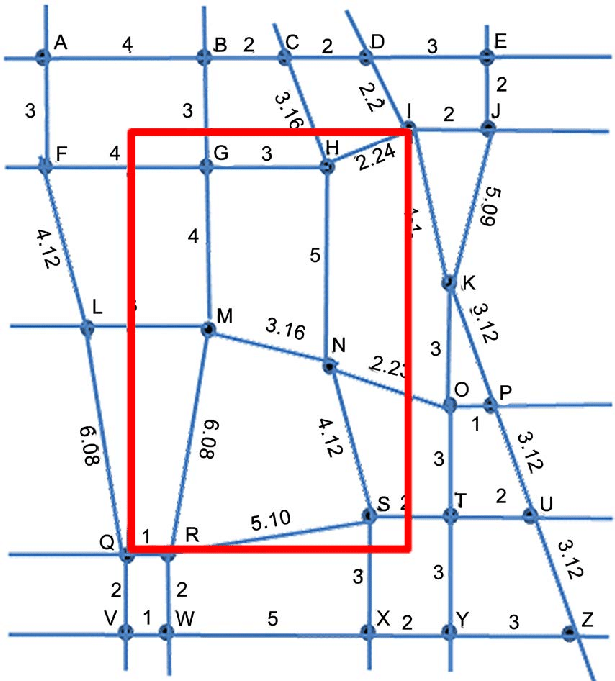
\includegraphics[width=0.9\linewidth]{images/bounding-box}
		\caption{Bounding box}
		\label{fig:boundingBoxReal}
	\end{subfigure}
	\begin{subfigure}[b]{0.48\textwidth}
		\centering
		\includegraphics[width=0.9\linewidth]{images/bounding-box-rect}
			\caption{Naklonený bounding box}
		\label{fig:boundingBoxRect}
	\end{subfigure}
	\caption[Bounding box]{}
	\label{fig:boundingBox}
\end{figure}

\begin{footnotesize}
Zdroj: Shortest Alternate Path Discovery through Recursive Bounding Box Pruning: Figure 5, Figure 13. Január 2017 [citované 18.8.2019]. Dostupné z \url{https://www.researchgate.net/publication/316188932_Shortest_Alternate_Path_Discovery_through_Recursive_Bounding_Box_Pruning}
\end{footnotesize}

\subsubsection{Navrhovaný algoritmus}
Dvojdimenzionálne súradnice v dopravnej sieti pomôžu určiť, či daný vrchol konverguje ku koncovému vrcholu alebo nie. 

Na začiatku vytvoríme \textit{bounding box} medzi začiatočným a koncovým vrcholom. Získame susedné vrcholy štartovného vrcholu a pre všetky susedné vrcholy vypočítame vzdialenosť $d$. Vzdialenosť $d$ je rovná súčtu vzdialenosti medzi štartovným vrcholom a daným susedným vrcholom a karteziánskou vzdialenosťou daného susedného vrcholu od koncového vrcholu. Zo susedných vrcholov je vybraný taký vrchol, ktorého hodnota $d$ je najmenšia. 

Nový vrchol sa stane začiatočným vrcholom a \textit{bounding box} sa znovu vygeneruje. Proces hľadania najbližšieho vrcholu pokračuje, kým sa najbližší vybraný vrchol nestane koncovým vrcholom. Týmto spôsobom nájdeme najkratšiu cestu. 

Následne vrcholy, ktoré sme nevyhodnotili, vyhodnotíme rovnakým spôsobom. Keď algoritmus spracuje všetky vrcholy, výsledok uloží vo vzostupnom poradí podľa veľkosti. Takto získame okrem najkratšej cesty aj alternatívne najkratšie cesty, viď obrázok \ref{fig:boundingBoxResult}. 

\begin{figure}[H]
\centerline{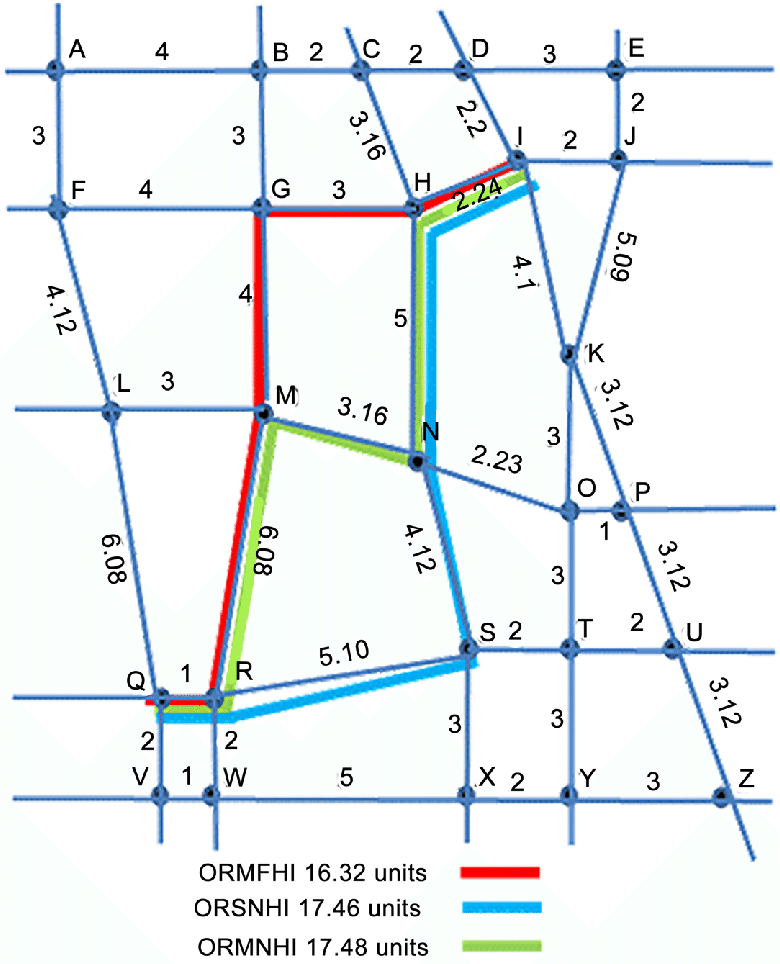
\includegraphics[width=0.4\textwidth]{images/bounding-box-result}}
\caption[Bounding box: 3 najkratšie cesty]{Bounding box: 3 najkratšie cesty}
\label{fig:boundingBoxResult}
\end{figure}

\begin{footnotesize}
Zdroj: Shortest Alternate Path Discovery through Recursive Bounding Box Pruning: Figure 5, Figure 12. Január 2017 [citované 18.8.2019]. Dostupné z \url{https://www.researchgate.net/publication/316188932_Shortest_Alternate_Path_Discovery_through_Recursive_Bounding_Box_Pruning}
\end{footnotesize}\\

Na záver vymeníme začiatočný vrchol s koncovým vrcholom a výsledné polia spolu zjednotíme, aby sme získali čo najlepší výsledok. 

V prípade, že algoritmu sa nepodarí nájsť najkratšiu cestu, rozšírime \textit{bounding box}. Maximálna výpočtová cena tohto algoritmu je $7 \cdot \sqrt{2}N$.

\subsection{Optimalizácia indexmi}
Autori článku \cite{IBAS} navrhli \textit{IBAS - Index-Based A-Star} algoritmus na vyriešenie problému najkratšej cesty pre ohodnotený graf, ktorého vrcholy nemajú reálne súradnice. Navrhli teda heuristiku, ktorá používa 3 indexy: 
\begin{itemize}
\item \textit{earlist arrival index} – predstavuje minimálnu cenu cesty zo začiatočného do koncového vrcholu
\item \textit{latest arrival index} – predstavuje maximálnu cenu cesty z koncového do začiatočného vrcholu
\item \textit{reverse earliest index} – predstavuje maximálnu cenu cesty zo začiatočného do koncového vrcholu
\end{itemize} 
Všetky indexy slúžia na určenie a odrezanie nepotrebných vrcholov pre výpočet najkratšej cesty, pričom \textit{earliest arrival index} je použitý na vytvorenie funkcie $f(n)$. 
Vytvorenie 3 indexov má zložitosť $\mathcal{O}(|V| + E|)$. IBAS používa A* algoritmus, takže zložitosť IBAS je o $\mathcal{O}(|V| + E|)$ horšia ako zložitosť A* algoritmu. Algoritmus je efektívny na statických dátach, kedy stačí vypočítať indexy pre každý vrchol len raz.


\section{Zohľadnenie zadania polohy mimo zástavky}
V článku \cite{circular} autori poukazujú na to, že väčšina miest má v rámci verejnej dopravy dva typy trás a to obojsmerné a okruhové. Odporúčajú, že v databáze je dobré ich nejakým spôsobom rozlíšiť, najmä kvôli výberu najbližšej zástavky k danej pozícii.

Správny systém na hľadanie optimálnej trasy vo verejnej doprave by mal ponúknuť používateľovi možnosť vyhľadať trasu z miesta/na miesto, ktoré nie je nutne zástavkou. Ak by sme hľadali najkratšiu cestu z takto zadaného vrcholu, prvým krokom bude nájdenie prvej zástavky. Autori upozorňujú na to, že vyhľadanie najbližšej zástavky k danej pozícii nemusí byť správnym riešením. Najmä pri dopravných sieťach s hustým rozsadením zastávok a pri okružných trasách.

Navrhujú nájsť viacero zástaviek radiálnym vyhľadávaním, ktorému určíme polomer. V mestách s hustým rozsadením zástaviek môže nastať taký problém, že vo vybranej zóne sa nachádza viac zástaviek, ktoré prislúchajú tej istej trase, ako môžeme vidieť na obrázku \ref{fig:circularRoute}. V tomto prípade by výber zástavky č. 1 (najbližšej zástavky k zadanej pozícii)  nebol optimálny. Rovnako aj vybratím zástavky č. 6 ako konečnej zástavky by nebolo súčasťou správneho riešenia hľadania najkratšej cesty. 

\begin{figure}[H]
\centerline{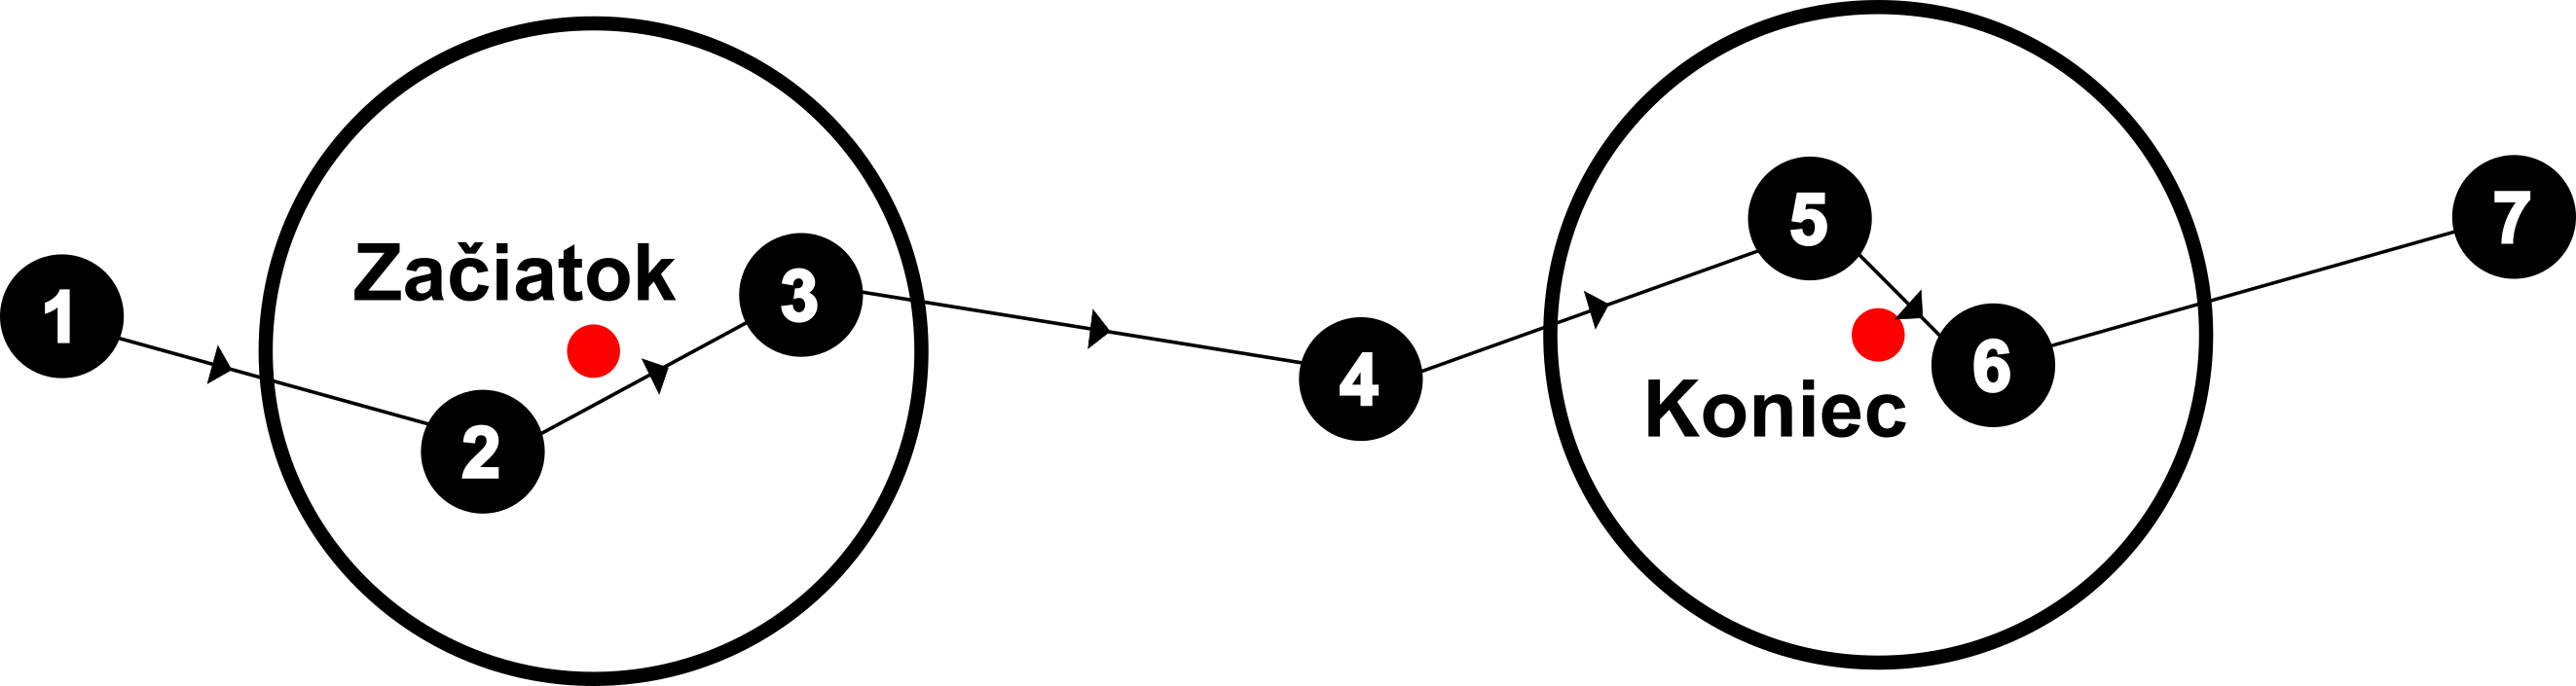
\includegraphics[width=0.6\textwidth]{images/circular-route}}
\caption[Okružná trasa]{Okružná trasa}
\label{fig:circularRoute}
\end{figure}

Autori článku navrhujú spôsob, ako správne vybrať zástavku, na ktorej nastúpiť a vystúpiť, aby bola dĺžka celkovej trasy čo najkratšia. Definujú \textit{closest stop C} ako najbližšiu zastávku k zadanému bodu. \textit{Least travelling stop L} je zástavkou, ktorá má pri hľadaní začiatočnej zástavky najväčšie poradové číslo alebo naopak najmenšie poradové číslo pri hľadaní konečnej zástavky. Rozhodný je rozdiel poradových čísel zástaviek \textit{C} a \textit{L}. V systéme definujeme hodnotu \textit{a} (alebo ju necháme zvoliť používateľom), ktorá predstavuje mieru ušetreného času na úkor dlhších peších presunov. Ak je rozdiel menší ako hodnota \textit{a}, vyberieme \textit{closest stop} a ak je väčší, vyberieme \textit{least travelling stop}. 

\section{Alternatívne optimálne cesty}
Pri hľadaní optimálnej cesty je potrebné zohľadniť, čo daný používateľ považuje za optimálne. Používateľ pri zadávaní vyhľadávacích parametrov nemusí poznať svoje preferencie alebo ich môže často meniť. Zadávanie preferencií pri každom vyhľadávaní nie je používateľsky prívetivé. Aby si napriek tomu používateľ mohol zvoliť cestu, ktorá najviac vyhovuje jeho potrebám, systém musí ponúknuť viac alternatívnych ciest. Tu sa dostávame k problému K najkratších ciest.

Ako tvrdia v článku \cite{dissimilar}, väčšina navigačných služieb neposkytuje používateľom viac ciest. A ak áno, využívajú algoritmus K najkratších ciest, ktorý poskytuje viacero alternatívnych ciest pre používateľa. Má však svoje obmedzenie. Často poskytuje alternatívne cesty, ktoré sú podobné vo veľkej časti úsekov. Mali by preto vyberať trasu s najmenšou spoločnou dĺžkou spomedzi tých, ktoré uspokojili povolené cestovné náklady.

Predstavili vývoj heuristického algoritmu, ktorý efektívne vyhľadáva rôzne alternatívne cesty. Algoritmus je popísaný vývojovým diagramom na obrázku \ref{fig:flowchart}.

\begin{figure}[H]
\centerline{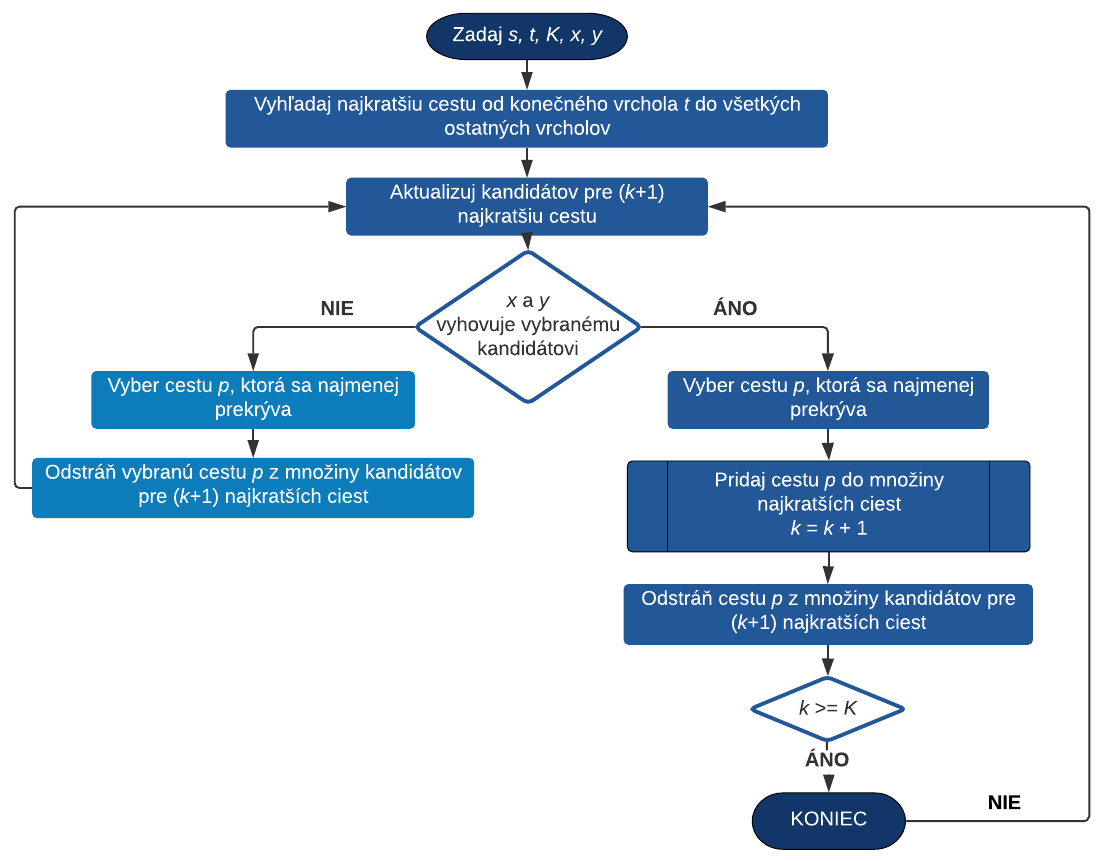
\includegraphics[width=0.6\textwidth]{images/flow-chart}}
\caption[Algoritmus - vývojový diagram]{Algoritmus - vývojový diagram}
\label{fig:flowchart}
\end{figure}
 

\section{Zohľadnenie krízových dopravných situácií}
Verejná doprava je u mnohých vnímaná ako nespoľahlivá, hoci sa podieľa na znižovaní dopravného zaťaženia. Výrazný vplyv na presnosť spojov a teda aj na kvalitu služieb verejnej dopravy majú práve krízové dopravné situácie. Nehody, rôzne poruchy spojov, plánované alebo aj neplánované údržbárske práce spôsobujú problémy vo verejnej doprave, ale aj pri navrhovaní systému.

V týchto okrajových prípadoch je o to dôležitejšie, aby systém zohľadnil všetky krízové situácie a ponúkol optimálnu cestu. Dnešné systémy väčšinou ponúkajú jednu alebo niekoľko trás, ktoré sú tvorené lineárnou postupnosťou úsekov a aktivít. Základné algoritmy na plánovanie optimálnej cesty predpokladajú deterministické prostredie. Vznikajú nové systémy, ktoré ponúkajú možnosť dynamického plánovania ciest a v prípade zmien upozornia cestujúceho a ponúknu opätovné naplánovanie cesty od pôvodného miesta podľa nových a aktuálnych dopravných podmienok. Lineárne plánovanie trasy nie je dostatočne flexibilné, pretože k opätovnému plánovaniu dôjde vždy po určitej odchýlke od predpokladaných pôvodných podmienok.

Autori článku \cite{routing} navrhujú použiť koncepciu \textit{routing policy} namiesto koncepcie lineárneho plánovania trasy.\textit{ Routing policy} určuje, ktorá služba sa má prijať v každej situácii. Pre dvojicu (zástavka, čas) špecifikuje zoznam služieb, ktoré sa odporúčajú cestujúcemu vykonať. Vždy existuje optimálna \textit{routing policy}, ale jej nájdenie predstavuje NP ťažký problém. Bol navrhnutý algoritmus, ktorý dokáže nájsť zoznam služieb v polynomiálnom čase obmedzením počtu odporúčaných služieb na každej zástavke v čase.

\section{Stavovo závislý algoritmus}
Hlavným rozdielom medzi stavovo závislým problémom hľadania najkratšej cesty a klasickým problémom hľadania najkratšej cesty je, že ohodnotenie hrán nie je konštanta, ale funkcia. Tým pádom nevieme na tento problém aplikovať klasické algoritmy hľadania najkratšej cesty. V článku \cite{trains} tvrdia, že ak dokážeme odhadnúť hodnotu hrany konštantným číslom, potom riešenie klasického problému hľadania najkratšej cesty môže fungovať ako heuristické riešenie problému najkratšej cesty závislej od stavu.

Toto riešenie aplikovali na Problém smerovania jedného vlaku. Cieľom je čo najrýchlejšie nasmerovať vlak cez prázdnu sieť s dvojkoľajovými úsekmi. Problém smerovania vlaku je NP ťažký. Bola navrhnutá heuristika dynamického programovania spolu s určitými podmienkami, aby heuristika mohla poskytnúť optimálne riešenie v polynomiálnom čase.

\section{Využitie stochastickej hodnoty}
Článok \cite{stochastic} poukazuje na to, že praktická doba jazdy po určitom úseku nie je v skutočnosti konštantná. Metóda navrhnutá na nájdenie optimálnej trasy v tomto článku je založená na stochastickom čase jazdy, ktorý môže správne opísať skutočnú dopravnú situáciu. Takéto metódy sa ale ťažko používajú v praxi, pretože získanie pravdepodobnostného rozdelenia času cestného úseku je náročné. V tomto výskume na získanie pravdepodobnostného rozdelenia používajú Bayesovu formulu.

Na zber údajov zvolili metódu Floating Car Data (FCD), ktorá účinne získava informácie o dopravnom toku v reálnom čase. 
Na analýzu stavu premávky sa používa priemerná rýchlosť jazdy. Nájsť optimálnu cestu na základne analytického riešenia niekoľkých integrálov je náročné. Preto na hľadanie optimálnej cesty navrhli a použili viaceré vylepšené genetické algoritmy. 
Z výsledkov praktickej analýzy vyplynulo, že navrhované metódy sú účinné pri riešení problému optimálnej cesty.

\section{Map - matching}
Na hľadanie optimálnej cesty vo verejnej doprave v reálnom čase potrebujeme reálne dáta o pohybe vozidiel. Tieto dáta môžeme získať v rôznej forme. V prípade, že získame len informáciu o pozícii vozidla z GPS, potrebujeme získané pozície vozidiel nejakým spôsobom spracovať. V článku \cite{mapmatching} navrhujú, ako spracovať takto získané dáta a následne nájsť najkratšiu cestu.

Proces \textit{map-matching} je metóda integrácie údajov z digitálnych máp s údajmi z polohovacieho systému (GPS). Tento proces slúži na identifikáciu správnej linky, po ktorej vozidlo ide a na určenie presnej polohy tohto vozidla v rámci linky. Na základe dostupnej geometrie cesty, topológie a charakteristiky polohových údajov použili rad matematických metód na získanie týchto informácií. 

Ďalej bol vyvinutý nový algoritmus \textit{stMM}, ktorý podporuje mapovanie nízkofrekvenčných údajov o polohe vozidla na mape. Jeho súčasťou je aj vyhľadávací A* algoritmus, ktorým hľadajú najkratšiu cestu medzi dvoma bodmi získanými s GPS. Pričom prihliadajú aj na možné prestupy medzi linkami a na obmedzenia pri odbočovaní na križovatkách.

Výsledky ukázali, že algoritmus identifikoval 98,9\% liniek správne a dokáže spracovať priemerne 50 aktualizácií polohy za sekundu.  
 

\section{RAPTOR algoritmus}
Doteraz spomínané algoritmy riešia problém hľadania optimálnej cesty vo verejnej doprave ako grafový problém. Ako sme uviedli v predchádzajúcich sekciách, najčastejšie sa pre tento problém vytvorí model dopravnej siete pomocou grafu a na ňom sa spustí algoritmus hľadania najkratšej cesty. Týmto riešením však väčšinou dostávame menej optimálne výsledky za vysoké výpočtové časy.

Techniky, ktoré sa opierajú o grafové modely ťažko spracovávajú dynamickosť v systémoch verejnej dopravy, ako časté meškanie liniek, náhle zrušenie liniek, zmeny trás a podobne. Hoci algoritmy hľadania najkratšej cesty sú rýchle, práve vytvorenie modelu spôsobuje spomínané vysoké výpočtové časy.

Autori článku \cite{raptor} predstavujú RAPTOR – Round-bAsed Public Transit Optimal Router, ktorý dokáže byť oveľa rýchlejší použitím jednoduchých obmedzovacích pravidiel a paralelizmu. Keďže RAPTOR algoritmus nepotrebuje žiadny grafový model, dokáže fungovať rýchlo a dynamicky. Pre dve zadané zastávky vráti všetky optimálne cesty s minimálnym časom príchodu do konečne zástavky a minimálnym počtom prestupov. Algoritmus beží v kolách a počíta časy príchodu prechádzaním jednotlivých trás.

Na rozdiel od grafových algoritmov, RAPTOR sa ľahko paralelizuje. Jednoducho rozdelí nezávislé linky medzi rôzne CPU jadrá. Existujú dve rozšírenia algoritmu a to McRAPTOR, ktorý zvláda riešiť viacero kritérií okrem času príchodu a počtu prestupov a rRAPTOR, ktorý vracia množinu ciest pre všetky odchody zo zastávky v danom časovom rozsahu. Bez potrebného pre-processingu a post-processingu dokáže spracovať aj kritérium preferovaných prestupných miest.

\subsection{Definície pojmov a premenných}

Definujeme cestovný poriadok ako $(\mathcal{S,T,R,F},\Pi)$, kde 
\begin{itemize}
\item $\Pi \subset \mathbb{N}_{0}$ je čas v sekundách, 
\item $\mathcal{S}$ je množina zastávok,
\item $\mathcal{T}$ je množina jázd, 
\item $\mathcal{R}$ je množina liniek a 
\item $\mathcal{F}$ je množina peších presunov.
\end{itemize}

Zástavka $p$ predstavuje miesto pre nastúpenie a vystpenie z vozidla. Môže to byť aj platforma. Jazda $t$ reprezentuje postupnosť zástavok konkrétneho vozidla. Každá zástavka $p$ z jazdy $t$ má priradený čas odchodu $\tau_{dep}(t, p) \in \Pi$ a čas príchodu $\tau_{arr}(t, p) \in \Pi$. Každá linka z $\mathcal{R}$ pozostáva z jázd, ktoré majú rovnaké postupnosti zastávok. Pešie prechody z množiny $\mathcal{F}$ reprezentujú prestupy medzi zástavkami. Každý prestup pozostáva z dvoch zastávok $p_1$ a $p_2$ a času potrebného na presun medzi nimi $l(p_1, p_2)$. 

Výstupom z algoritmu je cesta $\mathcal{J}$, ktorá je definovaná postupnosťou jázd a peších prestupov. Cesta, ktorá obsahuje $k$ jázd, má presne $k-1$ prestupov. Majme začiatočnú zastávku $p_s$ a konečnú zástavku $p_t$ a čas odchodu $\tau$. Najzákladnejším kritériom, na ktoré algoritmus prihliada, je \textit{Earliest Arrival Problem}, ktorý hľadá cestu nezačínajucú skôr než $\tau$ v bode $p_s$ a do $p_t$ sa dostane čo najrýchlejšie. Ďalej chceme viacero alternatívnych ciest s tým, že žiadna z ciest nezačína skorej ako $\tau$ a cesty môžu obsahovať aj prestupy. Cesta $\mathcal{J}_1$ dominuje nad cestou $\mathcal{J}_2$, ak platí
$\tau_{dep}(\mathcal{J}_1) \geq \tau_{dep}(\mathcal{J}_2)$ a $\tau_{arr}(\mathcal{J}_1) \leq \tau_{arr}(\mathcal{J}_2)$. 

\subsection{Základná verzia algoritmu}

Nech $p_s \in \mathcal{S}$ je začiatočný vrchol a $\tau \in \Pi$ je čas odchodu. Cieľom je vypočítať pre každé $k$ cestu do zástavky $p_t$ s minimálnym časom príchodu, ktorá je zložená z najviac $k$ jázd. Algoritmus beží v $k$ kolách. Kolo $k$ počíta najrýchlejšiu cestu do každej zastávky na $k-1$ prestupov. Niektoré zástavky nemusia byť dosiahnuteľné. Pri objasňovaní algoritmu bude počet kôl rovný $K$. Algoritmus pridelí každej zastávke $p$ postupnosť $(\tau_0(p), \tau_1(p), ..., \tau_K(p))$, kde $\tau_i(p)$ reprezentuje najskorší známy čas príchodu do zástavky $p$ na najviac $i$ jázd. 

Na začiatku sú všetky hodnoty vo všetkých postupnostiach pre každú zástavku inicializované na hodnotu $\infty$. Nastavíme $\tau_0(p_s) = \tau$. Dodržuje sa invariant: na začiatku kola $k$ je prvých $k$ hodnôt v postupnosti $\tau(p)$ správnych a ostatné hodnoty majú hodnotu $\infty$. Cieľom kola $k$ je vypočítať $\tau_k(p)$. Tento výpočet sa vykonáva v troch krokoch. 
 
V prvom kroku kola $k$ (ak $k \neq 0$) sa nastaví pre všetky zástavky $p$ hodnota $\tau_k(p) = \tau_{k-1}(p)$. Týmto nastavíme horné ohraničenie na najskorší príchod do zástavky $p$ na najviac $k$ jázd.

Druhé kolo spracuje práve raz každú linku $r$. Nech $\mathcal{T}(r) = (t_0, t_1, ..., t_{|\tau(r)|-1})$ je postupnosť jázd pre linku $r$ zoradená od najskôr začínajúcej po poslednú jazdu. Nach $et(r, p_i)$ je najskoršia jazda linky $r$, na ktorú je možné nastúpiť na zástavke $p_i$. Táto hodnota nemusí byť vždy definovaná. Pri spracovaní linky $r$ navštevujeme jej zástavky a hľadáme takú zástavku $p$, kde je hodnota $et(r, p_i)$ definovaná. Označme prislúchajúcu jazdu ako aktuálnu jazdu pre $k$. Ďalej prechádzame linku a pre každú zastávku $p_j$ aktualizujeme $\tau_k(p_j)$ použitím tejto jazdy. Aby sme vedeli spätné určiť výslednú cestu, nastavíme smerník na zastávku, na ktorej sme nastúpili na jazdu $t$. Navyše bude potrebné aktualizovať aktuálnu jazdu pre $k$. Na každej zo zastávok $p_i$ na linke $r$ môžeme stihnúť skoršiu jazdu, pretože sme v predchádzajúcich kolách mohli nájsť rýchlejšiu cestu do $p_i$. Je potrebné skontrolovať či $\tau_{k-1}(p_i) < \tau_{arr}(t, p_i)$ a aktualizovať $t$ prepočítané $et(r, p_i)$.

V treťom kroku zvažujeme pešie presuny. Zo zastávky $p_i$ sa môžeme dostať do niektorých zastávok peším presunom. Treba overiť, či týmto presunom nedosiahneme skorší čas príchodu do niektorej zo zastávok. Pre každý peší presun $(p_i, p_j) \in \mathcal{F}$ nastaví $\tau_k(p_j) = min\{\tau_k(p_j), \tau_k(p_i) + l(p_i, p_j)\}$. 

Algoritmus sa končí, keď po kole $k$ nebola vylepšená žiadna z hodnôt $\tau_k(p_i)$. 

Najhorší odhad časovej zložitosti algoritmu je lineárny, konkrétne $\mathcal{O}(K(\sum_{r \in \mathcal{R}} |r| + |\mathcal{T}| + |\mathcal{F}|)$, kde $K$ je počet kôl, pričom v každom kole $k$ prechádzame každú linku $r$ najviac jeden krát. Keďže $|r|$ je počet zastávok, spolu prechádzame $\sum_{r \in \mathcal{R}} |r|$ zastávok. Pri počítaní $et(r, p_i)$, prechádzame každú jazdu $t$ linky $r$ najviac jeden krát. 

\subsection{Optimalizácie algoritmu}
Pri hľadaní najkratšej cesty je prechádzanie všetkých liniek v každom kole zbytočné. V niektorých prípadoch neexistuje možnosť prestúpiť medzi dvoma linkami, takže niektoré z liniek sú nedosiahnuteľné. Majme linku $r$ a majme zástavku $p$ v $r$, ktorej posledné vylepšenie času príchodu bolo v kole $k' < k-1$. Linka $r$ bola opäť navštívená znovu v kole $k'+1 < k$, ale žiadnej z jej zastávok sa nevylepšil čas príchodu. Nie je dôvod prechádzať linku znovu, ak aspoň jedna z jej zastávok nebola vylepšená. 

Na implementáciu tejto optimalizácie postačí, ak si v kole $k-1$ označíme tie zástavky, pre ktoré bol v tomto kole vylepšený čas $\tau_{k-1}(p_i)$. Na začiatku kola $k$ prejdeme cez všetky tieto zástavky, označíme ich a nájdeme všetky linky, ktorým zastávky prislúchajú. Označené zástavky sú potenciálne miesta na prestup medzi linkami v kole $k$. Stačí nám dokonca prechádzať linku od prvej označenej zastávky v linke. Pridáme linky do pola $Q$ a zapamätáme si jej prvú označenú zastávku. 

Príklad môžeme vidieť na obrázku \ref{fig:raptor-optimal}. Algoritmus hľadá cestu zo zástavky $p_s$ do zástavky $p_t$. V prvom kole spracuje linku $r_1$, v druhom kole linky $r_2$ a $r_3$ a v treťom kole linku $r_4$. Iterovanie linky začína v prvej označenej zastávke linky (žltá farba). Zastávky označené bielou farbou nebudú po optimalizácii spracované v žiadnom kole. 

\begin{figure}[H]
\centerline{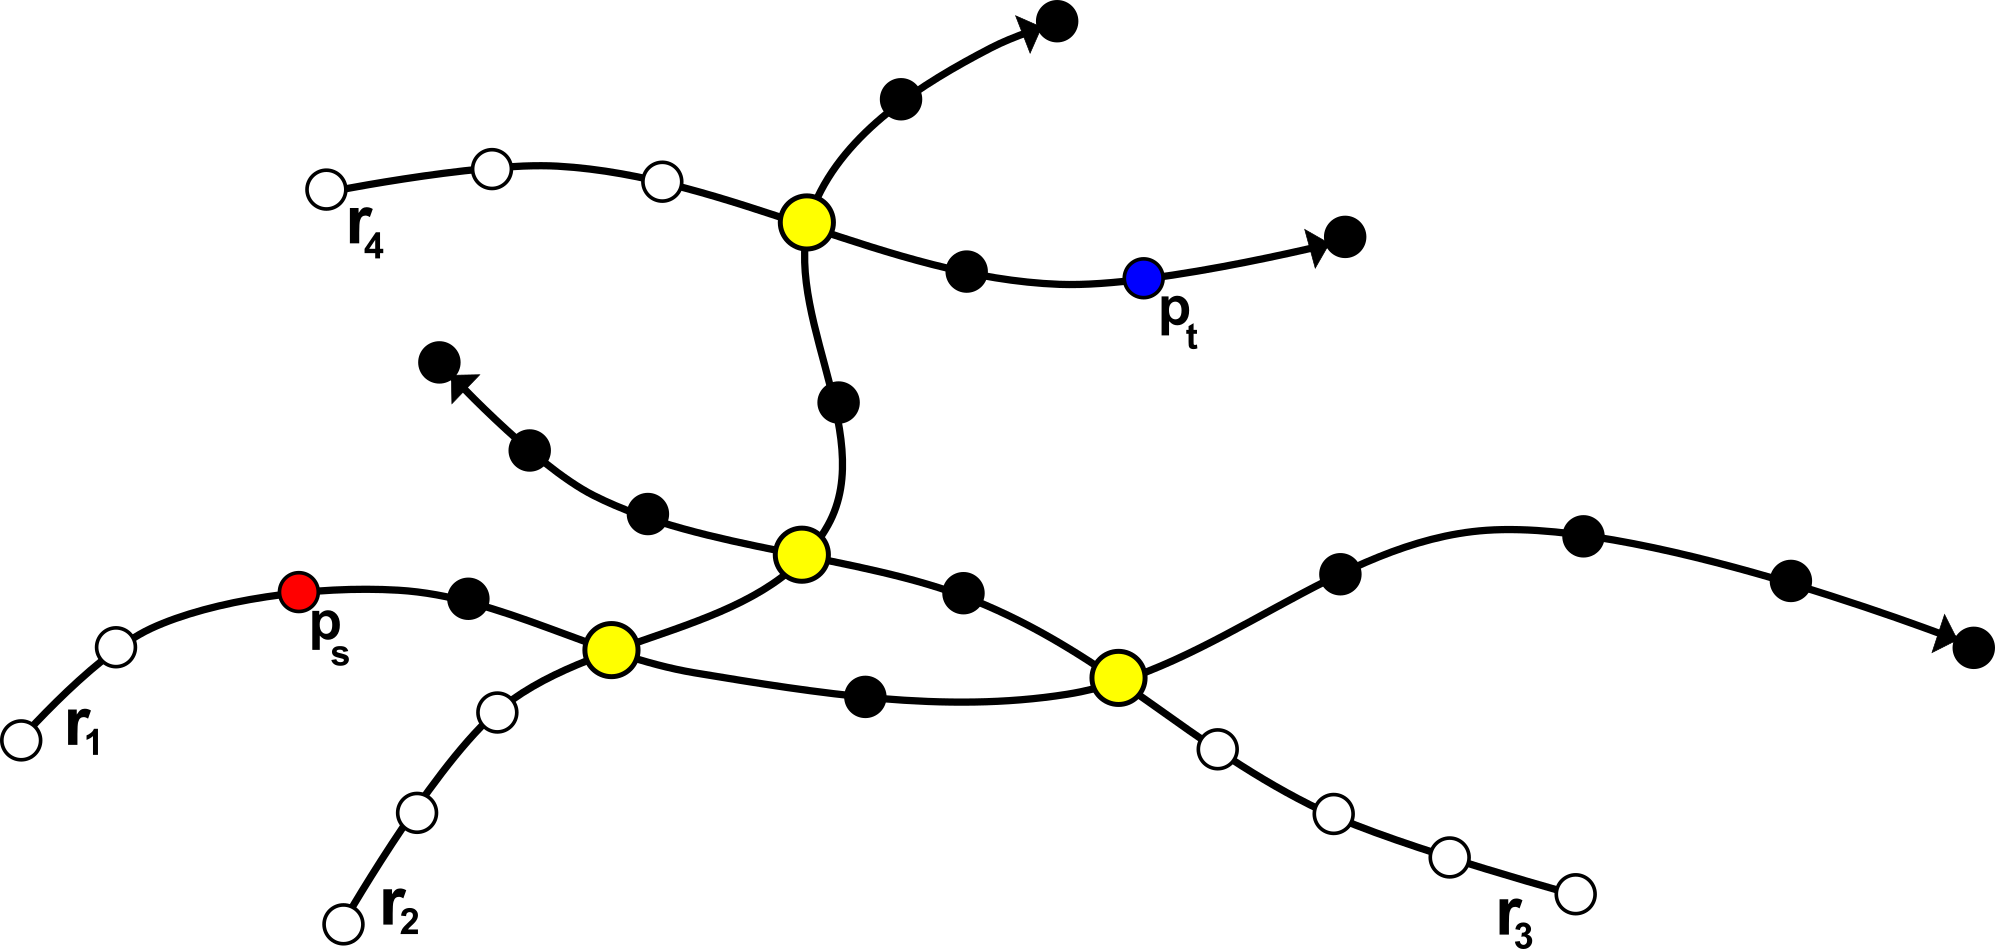
\includegraphics[width=0.9\textwidth]{images/raptor-optimal}}
\caption[RAPTOR - Optimalizácia prechádzania liniek]{RAPTOR - Optimalizácia prechádzania liniek}
\label{fig:raptor-optimal}
\end{figure}

Ďalšou optimalizačnou technikou je \textit{local prunning}. Pre každú zástavku $p_i$ si udržujeme hodnotu $\tau^*(p_i)$, ktorá reprezentuje najskorší známy čas príchodu na zástavku $p_i$. Vylepšením je, že zástavku označíme len v prípade, že čas príchodu v kole $k$ je menší ako predchádzajúca hodnota $\tau^*(p_i)$. 

RAPTOR algoritmus hľadá cestu zo začiatočnej zastávky do všetkých zastávok, hoci chceme nájsť cestu do konkrétnej konečnej zastávky. \textit{Target prunning} obmedzí hľadanie ciest do všetkých vrcholov na hľadanie jednej cesty. Dosiahneme to, ak v kole $k$ nebudeme označovať zastávky $p_i$, pre ktoré platí $\tau^*(p_i) > \tau^*(p_t)$.   

\subsection{Paralelizácia}
Ako sme si mohli všimnúť, linky sú individuálne a nie je potrebné ich iterovať v nejakom špecifickom poradí. Ak máme k dispozícii viac CPU jadier, každé z nich môže spracovávať inú podmnonžinu liniek. Nákladné môže byť zamedzenie prístupu do spoločného miesta v pamäti $(\tau_k(p))$. Autori navrhli 2 prístupy na riešenie paralelizácie bez využitia zámkov. Jeden prístup počíta s tým, že hardvér zaisťuje atomické zapisovanie do pamäte a druhý sa zaobíde aj bez tejto možnosti. 

\subsection{Dátová štruktúra}
Autori článku navrhli aj štruktúru, ktorá je vhodná pre RAPTOR algoritmus. Linky, jazdy a zastávky indexujeme od $0$. Potrebujeme pole liniek \textit{Routes}, ktoré si pre každú linku $r_i$ uchováva informáciu o počte zastávok na linke $r_i$ a smerník na pole \textit{RouteStops}, ktorý označuje začiatok postupnosti zastávok na linke $r_i$. Podobne aj pre jazdy si linka $r_i$ uchováva smerník, ktorý ukazuje na začiatok bloku v poli \textit{StopTimes}. Jeden blok v poli \textit{StopTimes} obsahuje všetky jazdy prislúchajúce linke $r_i$ zoradené podľa času odchodu z prvej zastávky. Každú jazdu reprezentuje postupnosť časov (čas príchodu a čas odchodu). Štruktúra ja zobrazená na obrázku \ref{fig:raptor-structure}. 

\begin{figure}[H]
\centerline{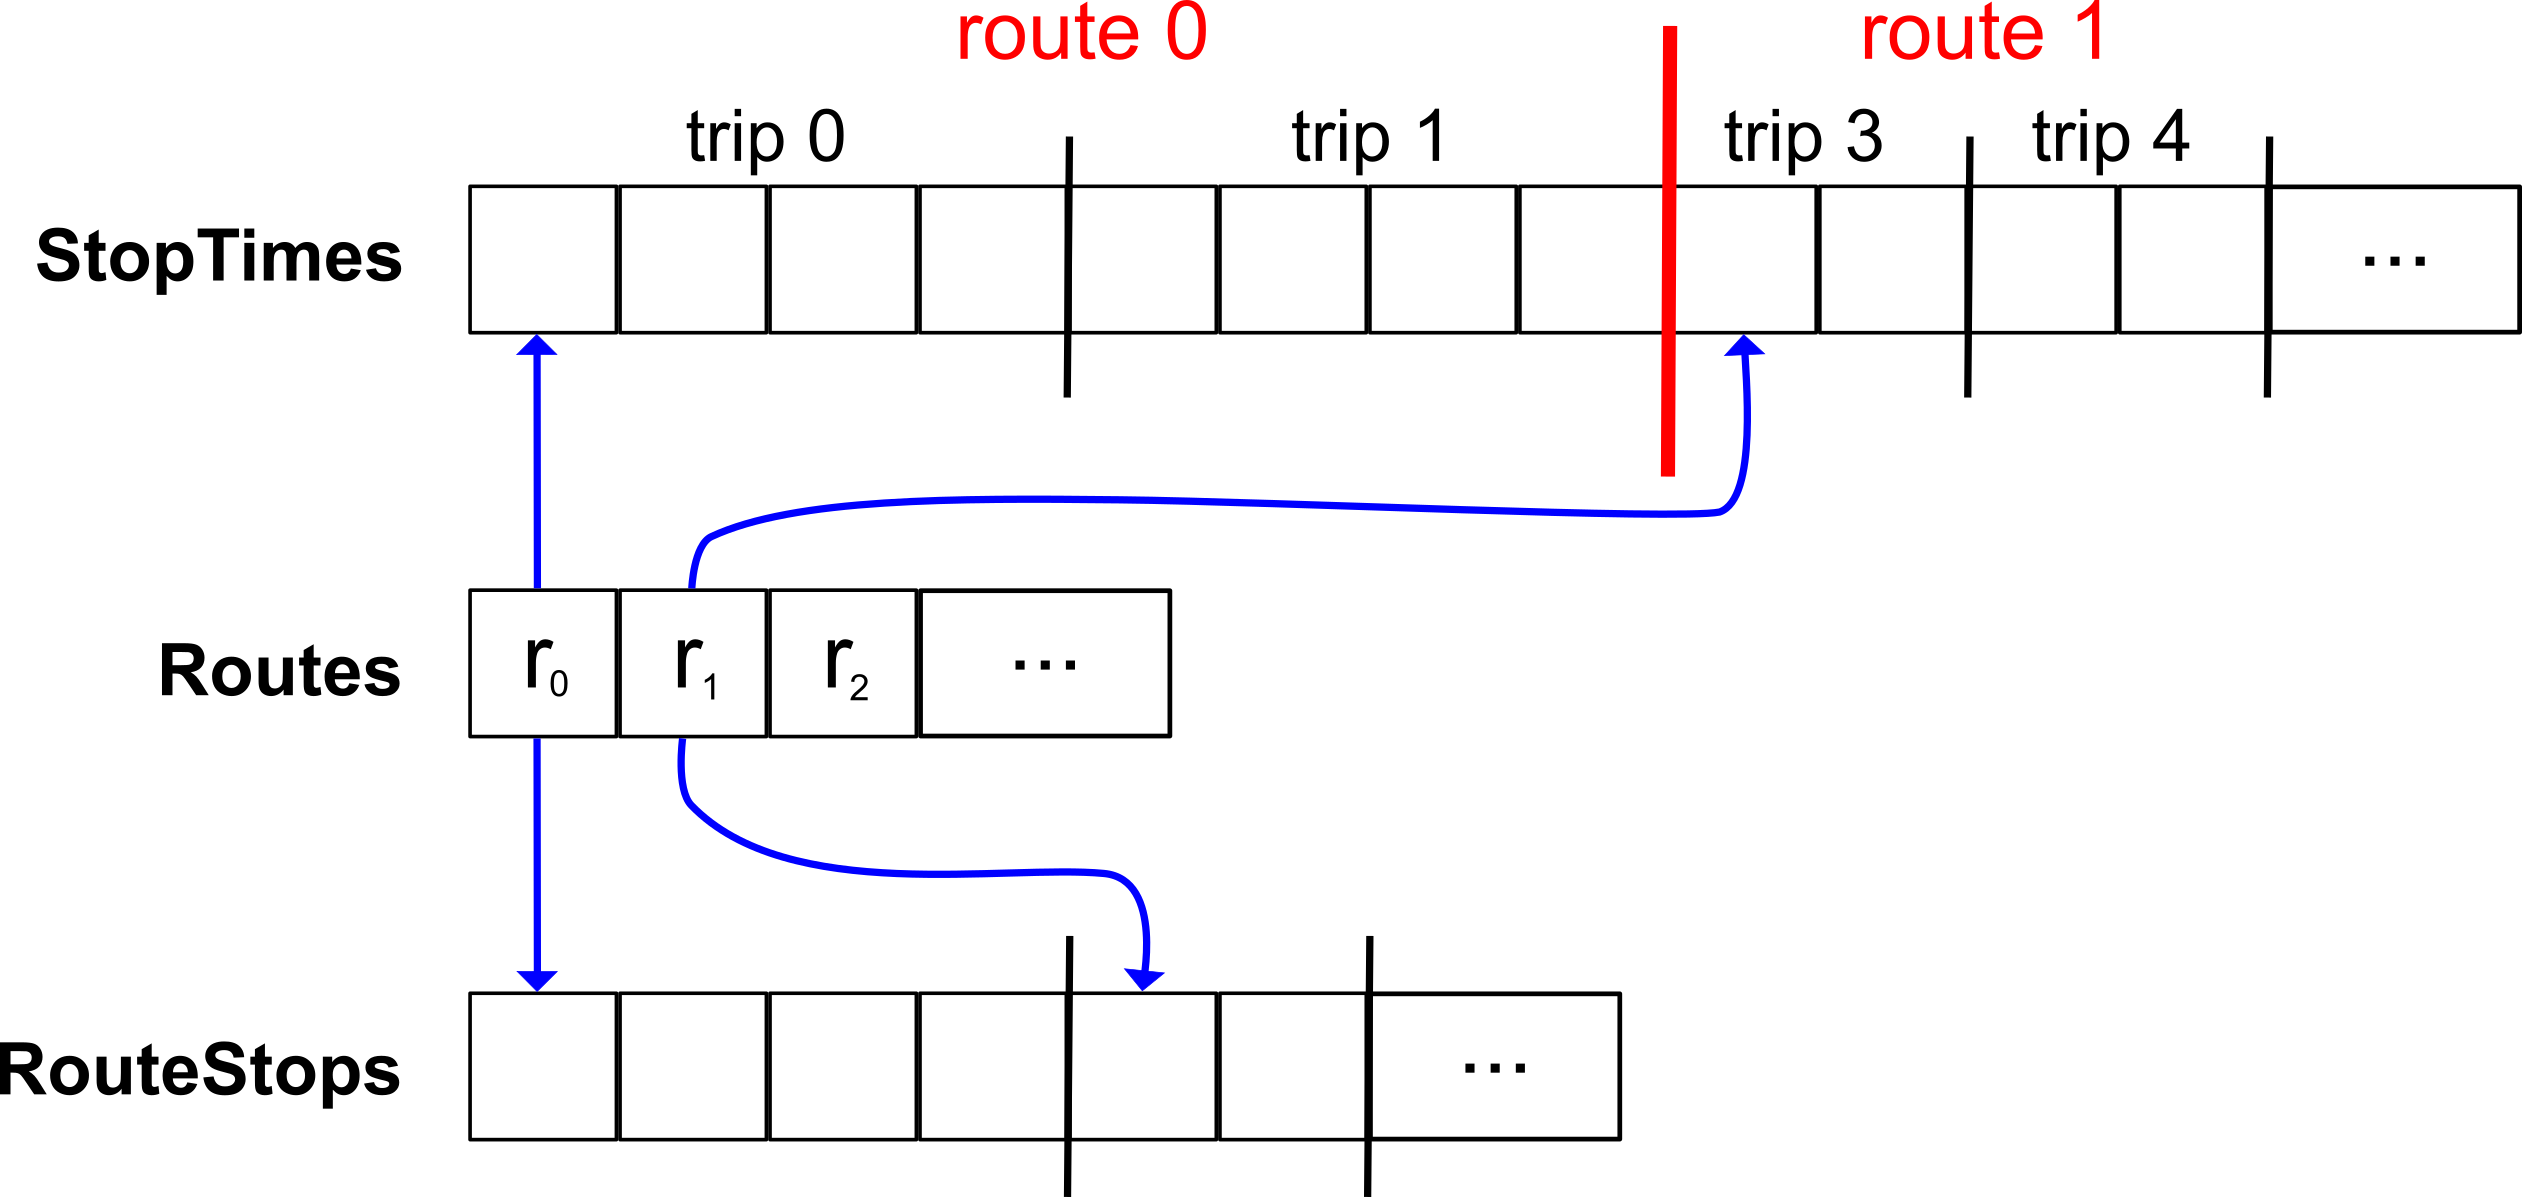
\includegraphics[width=0.7\textwidth]{images/raptor-structure}}
\caption[RAPTOR - Dátová štruktúra]{RAPTOR - Dátová štruktúra}
\label{fig:raptor-structure}
\end{figure}

V algoritme často potrebujeme iterovať cez zastávky linky $r_i$. Na to nám slúži pole \textit{RouteStops}. Ak potrebujeme získať najskorší čas odchodu zo zastávky $p$ po čase $\tau$, spôsob akým je pole \textit{StopTimes} utriedené nám zabezpečí, že čas tejto operácie bude konštantný.
Pri kontrolovaní, či sa v predchádzajúcej jazde nezlepšil čas odchodu niektorej zo zastávok, potrebujeme preskočiť na predchádzajúcu jazdu v poli \textit{StopTimes}. Na urýchlenie tejto operácie máme uloženú informáciu o počte zastávok pre linku $r_i$.

Takto navrhnutá štruktúra nie je pre algoritmus dostatočná. Na zohľadnenie prestupov potrebujeme ďalšie štruktúry a to pole \textit{Stops}, ktoré obsahuje všetky zastávky. Ďalej pole \textit{StopRoutes}, ktoré má pre každú zastávku priradené linky, ktoré na nej zastavujú. Pole \textit{Transfers}, ktoré obsahuje informácie o peších prechodoch medzi zastávkami. Pre každú zastávku je priradená dvojica: cieľová zastávka a čas potrebný na peší presun na túto zastávku. Náčrt doplňujúcej dátovej štruktúry je na obrázku \ref{fig:raptor-structure2}.

\begin{figure}[H]
\centerline{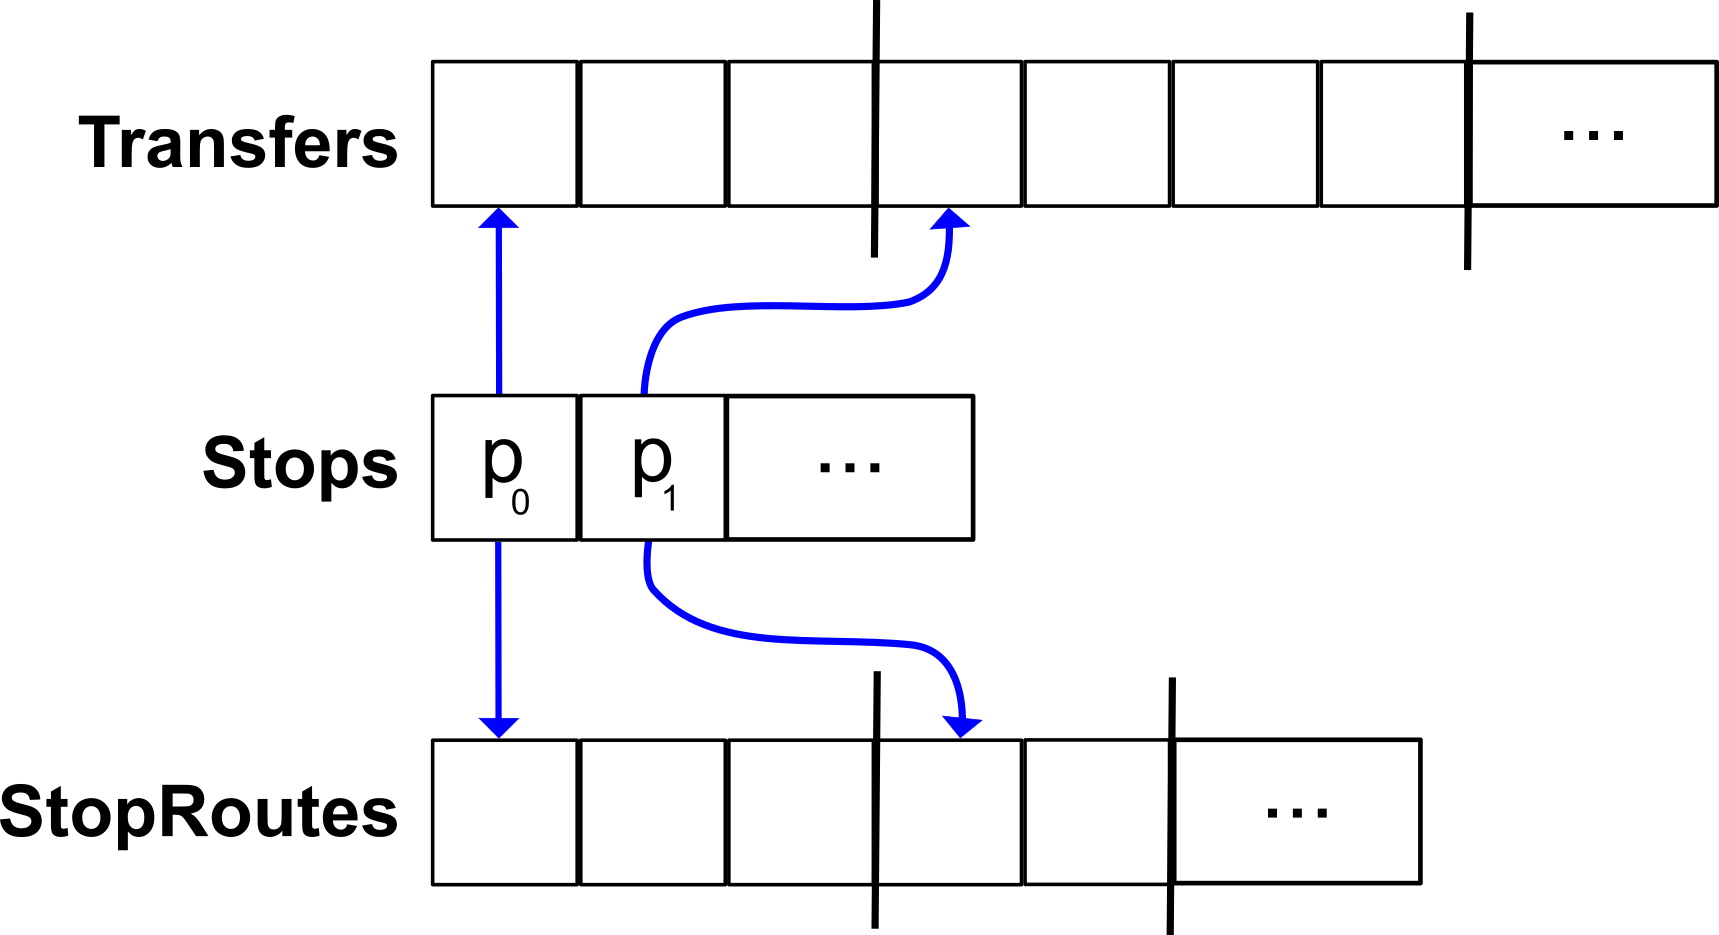
\includegraphics[width=0.5\textwidth]{images/raptor-structure2}}
\caption[RAPTOR - Dátová štruktúra na zohľadnenie prestupov]{RAPTOR - Dátová štruktúra na zohľadnenie prestupov}
\label{fig:raptor-structure2}
\end{figure}

\subsection{Vylepšený RAPTOR algoritmus}
Za výslednú cestu považoval RAPTOR algoritmus tú cestu, ktorá stojí najmenej času nezávisle od toho, koľko prestupov vyžaduje. Keďže cestujúci v skutočnosti nepreferujú cesty s veľkým počtom prestupov, je potrebné zaviesť do algoritmu ich penalizáciu. Ako sme už spomínali v predchádzajúcich sekciách, v prípade verejnej dopravy, ktorá ma viacero módov je nutné vyhľadať a ponúknuť cestujúcemu viacero alternatívnych ciest. Pôvodný RAPTOR algoritmus vracia len jednu najkratšiu cestu. 

V článku \cite{improvedRaptor} bol navrhnutý vylepšený RAPTOR algoritmus, ktorý má v sebe zapracovanú penalizáciu prestupov, korekčný faktor peších prestupov a vracia $k$ alternatívnych ciest. Cesty vypočítané vylepšeným algoritmom sa oveľa viac podobajú cestám, ktoré si v realite cestujúci vyberajú.

V tomto článku nám pribudlo označenie $k$-tej najkratšej cesty. Kedže písmenom $k$ sme doteraz označovali kolá, budeme hľadať $m$-tú najkratšiu cestu. Taktiež pribudli nové označenia a premenné, ktoré sú uvedené v tabuľke \ref{table:raptor-variables}.

\begin{table}[H]
\begin{tabular}{|l|l|}
\hline
\rowcolor[HTML]{C0C0C0} 
\textbf{Premenná} & \textbf{Popis} \\ \hline
$t_r$             & jazda $t$ linky $r$          \\ \hline
$Tr_c$             & penalizácia prestupu typu $c$          \\ \hline
$l(p, p_i)$       & čas pešieho prestupu zo zastávky $p$ do zastávky $p_i$ \\ \hline
$\tau_k(p)$			& najskorší známy čas príchodu na zastávku $p$ v $k$ kolách \\ \hline
$\tau_k(t, p)$    & najskorší známy čas príchodu na zastácku $p$ použitím jazdy $t$ v $k$ kolách \\ \hline
$\mathcal{J}_k(p)$ & množina ciest, ktorými sa viam dostať na zastávku $p$ v $k$ kolách \\ \hline
$\mathcal{J}_{k,m}(p)$ & $m$-tá najskoršia cesta, ktorou sa viem dostať na zastávku $p$ v $k$ kolách \\ \hline
$\mathcal{J}_k(p, p_i)$ & cesta zo zastávky $p$ do zastávky $p_i$ v $k$ kolách \\ \hline
\end{tabular}
\caption{Tabuľka premenných pre vylepšený RAPTOR algoritmus}
\label{table:raptor-variables}
\end{table}

\subsubsection{Penalizácia prestupov}
Penalizácia prestupov je pojem zahŕňajúci časové a nečasové prvky prestupu. Medzi časové prvky patrí čakanie na prestupný spoj a čas potrebný na peší presun. Načasovými prvkami môže byť pohodlie a komplikovanosť prestupu, ktoré závisia najmä od toho, či prestupujeme medzi rovnakými módmi alebo sa módy líšia. 

Autori článku definujú dva druhy prestupov: horizontálny a vertikálny. Napríklad prestup medzi autobusmi je horizontálny, ale pri prestupe z autobusu na metro je potrebné použiť schody a preto sa jedná o vertikálny prestup. Podľa druhu prestupu $c$ aplikujeme penalizáciu prestupu $Tr_c$. Pri implementácii si potrebujeme pamätať predchádzajúci mód jazdy, ktorým cestujúci prišiel na zastávku, na ktorej bude prestupovať.

Čo sa týka času potrebného na peší presun medzi jednotlivými zastávkami, priemerná rýchlosť kráčania dospelého človeka bola určená na $1.2 m/s$. Väčšinou sa predpokladá, že dĺžka prestupu je Euklidovská vzdialenosť od počiatočnej zastávky po cieľovú. Tento odhad ale nie je vyhovujúci, pretože vo väčšine prípadov je trasa prestupu dlhšia ako vzdušná čiara medzi zastávkami. Navrhli preto použiť Manhattanovskú vzdialenosť. Keď je vzdialenosť vzdušnou čiarou rovná 1, Manhattanovská vzdialenosť má hodnotu $\sqrt{2}$.

\subsubsection{Hľadanie viacerých ciest}
Vylepšený algoritmus hľadá $M$ najkratších ciest. Je potrebné zabrániť tomu, aby v rámci $m$-nájdených ciest boli podobné cesty. Autori navrhli 2 pravidlá, použitím ktorých zabránia výskytu podobných ciest vo výsledných $M$ cestách.

Prvým pravidlom je, že jazda $t$ linky $r$ by sa už znova nemala vyhľadať zo zastávky, na ktorej cestujúci vystúpi. Príklad je na obrázku \ref{fig:similar-paths}(a). Červená cesta vedie priamo zo začiatočnej zastávky $S$ do konečnej zastávky $T$ a modrá cesta obsahuje navyše prestup na zastávke $A$. Časy príchodu týchto dvoch ciest sa líšia a preto by sa cesty vyhodnotili ako rôzne. Týmto zabránime tomu, aby červená a modrá cesta boli vybrané súčasne.

Druhé pravidlo považuje cesty za podobné, ak je postupnosť zastávok v oboch cestách rovnaká. Na obrázku \ref{fig:similar-paths}(b) môžeme vidieť, že cesty sa líšia v mieste prestupu a tým pádom aj v čase príchodu do cieľovej zastávky. Preto by tieto cesty boli vyhodnotené ako rozdielne. Po aplikovaní pravidla budú vyhodnotené ako podobné. 
V $\mathcal{J}_k(p)$ sú uložené cesty, ktorými sme sa dostali na zastávku $p$ v kole $k$. Ak prídeme na zastávku $p$ v čase $\tau_k(p)$, porovnáme časy príchodov už existujúcich ciest z množiny $\mathcal{J}_k(p)$ a len tá s minimálnym časom príchodu bude aktualizovaná.

\begin{figure}[H]
\centerline{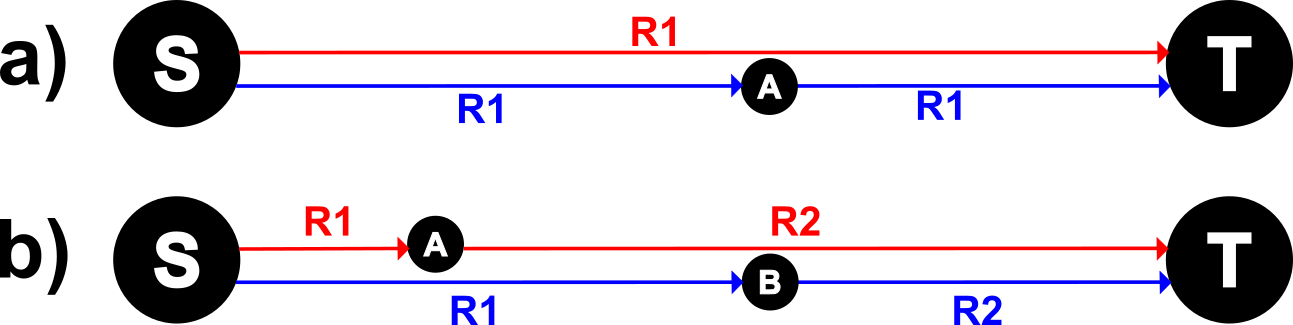
\includegraphics[width=0.7\textwidth]{images/similar-paths}}
\caption[RAPTOR - podobné cesty]{RAPTOR - podobné cesty}
\label{fig:similar-paths}
\end{figure}

Ďalej je popísaný algoritmus \ref{alg:1}, ktorý zhodnotí, či je cesta $\mathcal{J}_k(p, p_i)$ podobná ako niektorá z ciest zaznamenaných v množine $\mathcal{J}_k(p_i)$.

\begin{algorithm}
\caption{Algoritmus na zistenie podobných ciest}\label{alg:1}
 \hspace*{\algorithmicindent} \textbf{Input: $\mathcal{J}_k(p_i)$, $t_r$, $\mathcal{J}_k(p, p_i)$} \\
 \hspace*{\algorithmicindent} \textbf{Output: true or false} 
\begin{algorithmic}[1]
\ForEach{$\mathcal{J}_{k,m}(p_i) \in \mathcal{J}_k(p_i)$}
\If {last $t$ of $\mathcal{J}_{k,m}(p_i) = t_r$} \Return false
\ElsIf { $\mathcal{J}_k(p, p_i) = \mathcal{J}_{k,m}(p_i)$} \Return false
\Else {} \Return true
\EndIf
\EndFor
\end{algorithmic}
\end{algorithm}

\subsubsection{Zhrnutie vylepšeného RAPTOR algoritmu}
Algoritmus nám vráti $M$ najskorších ciest, ktoré vedú na zastávku $p_t$. Vstupom pre algoritmus je čas odchodu $\tau$, začiatočná zastávka $p_s$ a konečná zastávka $p_t$. Začíname v kole $m=0$. Pre každú zastávku $p$ nastavíme hodnotu $\tau_k(p)=\infty$, okrem začiatočnej zastávky $p_s$. Tá bude mať hodnotu $\tau_k(p_s)=\tau$ a bude označená.
\\
\\
\textbf{KROK 1:} Ak nie sme v kole $0$, pre každú zastávku $p$ nastavíme $\tau_k(p) = \tau_{k-1}(p)$ a $\mathcal{J}_k(p)=\mathcal{J}_{k-1}(p)$.\\
\textbf{KROK 2:} Pre každú zastávku $p$ označenú v kole $k-1$ hľadáme všetky zastávky $p_i$, na ktoré sa vieme dostať peším presunom zo zastávky $p$. Ak $\tau_k(t, p)$ cesty $\mathcal{J}_k(p, p_i)$ je skôr ako $\tau_k(p_i)$, tak do $\tau_k(p_i)$ vložíme hodnotu $\tau_k(t, p)$ a označíme zastávku $p_i$. Ak počet ciest v množine $\mathcal{J}_k(p_i) < K$, pridaj cestu $\mathcal{J}_k(p, p_i)$ do tejto množiny. Ak je veľkosť množiny rovnaká ako $K$, nahraď cestu $\mathcal{J}_{k,m}(p_i)$ cestou $\mathcal{J}_k(p, p_i)$ a označ zastávku $p_i$. Ak nastane nejaká zmena v množine $\mathcal{J}_k(p_i)$, zotrieď ju podľa času príchodu do zastávky $p_i$. \\
\textbf{KROK 3:} Pre každú označenú zastávku $p$, vložíme všetky dvojice $(r, p)$ do poľa $Q$, pričom platí, že linka $r$ obsluhuje zastávku $p$.\\
\textbf{KROK 4:} Pre každú dvojicu $(r, p)$ hľadáme jazdu $t_r$, ktorá príde na zastávku $p$ po čase $\tau_k(p) + Tr_c$.\\
\textbf{KROK 5:} Ak je posledná linka v množine $\mathcal{J}_{k,m}(p)$ identická s linkou $r$, preskoč KROK 6 a KROK 7.\\
\textbf{KROK 6:} Hľadaj jazdu $t_r$ linky $r$ a pre každú zastávku $p_i$, ktorá patrí tejto linke over, či existuje podobná cesta ceste $\mathcal{J}_k(p, p_i)$. Ak už podobná cesta existuje, pokračuj KROKOM 7. Inak, ak počet ciest v $\mathcal{J}_k(p_i) < K$, pridaj cestu $\mathcal{J}_k(p, p_i)$ do tejto množiny. Ak je veľkosť množiny rovnaká ako $K$, porovnaj čas $\tau_k(p_i)$ cesty $\mathcal{J}_{k,m}(p_i)$ s časom $\tau_k(t, p)$ cesty $\mathcal{J}_k(p, p_i)$. Ak je čas $\tau_k(t,p)$ menší, nahraď $\mathcal{J}_{k,m}(p_i)$ cestou $\mathcal{J}_k(p, p_i)$ a označ zastávku $p_i$.  Ak nastane nejaká zmena v množine $\mathcal{J}_k(p_i)$, zotrieď ju podľa času príchodu do zastávky $p_i$. \\
\textbf{KROK 7:} Nájdi cestu, ktorá má rovnakú postupnosť liniek akú má $\mathcal{J}_k(p, p_i)$ a ak platí $\tau_k(t, p)$ cesty $\mathcal{J}_k(p, p_i)$ < $\tau_k(p_i)$ cesty $\mathcal{J}_{k,m}(p_i)$, tak aktualizuj $\tau_k(p)$, označ zastávku $p_i$ a zotrieď množinu $\mathcal{J}_k(p_i)$\\
\textbf{KROK 8:} Ak existuje zastávka, ktorá má hodnotu $\tau_k(p)$ aktualizovanú v kole $k$, pokračuj v algoritme znovu od KROKU 1. Inak ukonči proces.

 
\section{Architekúra systému}
Správne navrhnutie architektúry systému je kľúčové pre efektívny beh aplikácie, najmä pri systémoch, kde sa dáta neustále menia. Problém s architektúrou analyzujú aj pri navigačných systémoch napríklad v článku \cite{onlineSP}. Tvrdia, že klasická klient-server architektúra pre online výpočet najkratšej cesty sa zle prispôsobuje veľkému počtu klientov. Ide o architektúru, kedy klient (navigačný systém) posiela dopyt na server a čaká na odpoveď. Počet zariadení stále pribúda a tak tento model čelí obmedzeniam ako šírka pásma siete a načítanie servera.

Autori článku sa inšpirujú riešením - \textit{index transmission model}. Tento model spočíva vo vysielaní indexu cez bezdrôtovú sieť, kedy si každý klient sťahuje len časť celej mapy, podľa informácii indexu. \textit{Index transmission model} síce rieši problém s počtom klientov, ale neznižuje množstvo nákladov potrebných na aktualizáciu indexu podľa reálnej dopravnej situácie.

Predstavujú \textit{LTI - Live Traffic Index} ako hlavný technický postup. Cestný monitorovací systém pozostáva z \textit{traffic provider} (Google Maps, NAVTEX, ...), \textit{service provider} a veľkého množstva mobilných klientov, ako je zobrazené na obrázku \ref{fig:LTIsystm}. \textit{Traffic provider} zbiera informácie o aktuálnej dopravnej situácii z cestných senzorov a video analýz. \textit{Service provider} pravidelne prijíma aktuálne dopravné zmeny od \textit{traffic providera}. Na začiatku vytvorí štruktúru indexu (grafu) a udržiava ju podľa aktuálnych dopravných okolností. Vytvorenie štruktúry indexu je jednorazová akcia. Potom sa index rozdelí na množinu podgrafov, aby boli pripravené na vysielanie. Hierarchickú indexovú štruktúru optimalizovali technikou \textit{graph partitioning} a stochastickými konštrukciami.

\begin{figure}[H]
\centerline{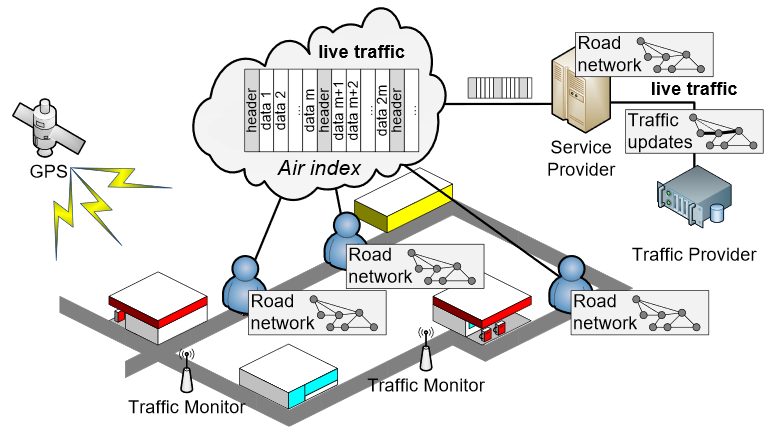
\includegraphics[width=0.6\textwidth]{images/onlineSP}}
\caption[LTI sysém]{LTI sysém}
\label{fig:LTIsystm}
\end{figure}

\begin{footnotesize}
Zdroj: Towards Online Shortest Path Computation: Figure 3. December 2013 [citované 25.8.2019]. Dostupné z \url{https://ieeexplore.ieee.org/abstract/document/6678359/figures#figures}
\end{footnotesize}\\

Na serveri sa index musí udržovať vždy aktualizovaný. Na riešenie aktualizácie hrany navrhli použitie dynamického Dijkstrovho algoritmu a \textit{DSPT - dynamic shortest path tree}. 

Výpočet najkratšej cesty sa vykonáva na klientskej strane. Štruktúra grafu je distribuovaná každému klientovi vopred mesačnými aktualizáciami alebo pri zavádzaní systému. Klient potrebuje aktualizovať len určitú časť grafu, ktorú potrebuje na výpočet najkratšej cesty. 

Keď server vysiela súbor údajov, všetci klienti sa potrebujú pripojiť a počúvať súčasne. Na dosiahnutie tohto cieľa používajú \textit{(1, m) interleaving} schému. Táto schéma je protokolom medzi klientom a serverom. Klient sa pripojí na vysielací kanál a počúva, kým nezíska segment hlavičky. Segment obsahuje ohodnotenia príslušných častí grafu. Po prečítaní segmentu rozhoduje, či tieto ohodnotenia potrebuje alebo nie. Ak áno, aktualizuje graf a vypočíta najkratšiu cestu. Pri aktualizácii sa menia len ohodnotenia, nie celá štruktúra grafu.


